\documentclass{article}

\usepackage{defines}

\begin{document}

\tickettitle{10}{Понятие скалярного произведения векторов. Четыре свойства скалярного произведения с доказательствами. Теорема о скалярном произведении в аффинной системе координат. Следствия о модуле вектора и угла между векторами через скалярное произведение.}

\define{угла между векторами}

\begin{minipage}{0.6\linewidth}
	Углом между векторами $\vec{a}$ и $\vec{b}$ называются угол $<\pi$, который они образуют после приведения их в общее начало.
	\begin{enumerate}
		\item{}Приведём $\vec{a}$ и $\vec{b}$ к общему началу $O$
		\item{}$A:\lvec{OA}=\vec{a}$
		\item{}$B:\lvec{OB}=\vec{b}$
	\end{enumerate}
	\begin{align*}
		\angle(\vec{a},\vec{b}):=\angle AOB
	\end{align*}
\end{minipage}%
\begin{minipage}{0.4\linewidth}
	\centering
	\begin{tikzpicture}
		\coordinate (O) at (0,0) node[anchor=east] at (O) {$O$};
		\coordinate (A) at (3,1) node[anchor=north] at (A) {$A$};
		\coordinate (B) at (1,3) node[anchor=west] at (B) {$B$};
		\draw [-latex] (O)--(A) node[midway, above] {$\vec{a}$};
		\draw [-latex] (O)--(B) node[midway, left] {$\vec{b}$};
		\draw [domain=18.5:71.5] plot ({cos(\x)},{sin(\x)});
	\end{tikzpicture}
	\captionof{figure}{Угол между векторами}
\end{minipage}

\define{скалярного произведения векторов}

Скалярное произведение векторов $\vec{a}$ и $\vec{b}$ обозначается как $(\vec{a},\vec{b})$ или $\vec{a}\cdot\vec{b}$
\begin{align*}
	(\vec{a},\vec{b}):=|\vec{a}||\vec{b}|\cos\angle(\vec{a},\vec{b})
\end{align*}
\begin{align*}
	 & (\vec{a},\vec{a})=|\vec{a}||\vec{a}|=|\vec{a}|^{2} &  & \cos\angle(\vec{a},\vec{b})=\frac{(\vec{a},\vec{b})}{|\vec{a}||\vec{b}|}
\end{align*}

\sectitle{Свойства скалярного произведения}

\theorem[о коммутативности скалярного произведения]
\begin{align*}
	(\forall \vec{a},\vec{b}\in L)\;(\vec{a},\vec{b})=(\vec{b},\vec{a})
\end{align*}

\proof
\begin{align*}
	(\vec{a},\vec{b})=|\vec{a}||\vec{b}|\cos\angle(\vec{a},\vec{b})=|\vec{b}||\vec{a}|\cos\angle(\vec{a},\vec{b})=(\vec{b},\vec{a})\qed
\end{align*}

\theorem[об ассоциативности скалярного произведения]
\begin{align*}
	(\forall \lambda\in\R, \vec{a},\vec{b}\in L)\;(\lambda\vec{a},\vec{b})=\lambda(\vec{a},\vec{b})
\end{align*}

\proof
\begin{align*}
	 & \begin{cases}
		   \lambda\vec{a}\upuparrows\vec{a}   & \text{при }\lambda>0 \\
		   \lambda\vec{a}\updownarrows\vec{a} & \text{при }\lambda<0 \\
	   \end{cases}\Rarr
	\begin{cases}
		\cos\angle(\lambda\vec{a},\vec{b})=\cos\angle(\vec{a},\vec{b})    & \text{при }\lambda>0 \\
		\cos(\angle(\lambda\vec{a},\vec{b}))=-\cos\angle(\vec{a},\vec{b}) & \text{при }\lambda<0 \\
	\end{cases}\Rarr\cos\angle(\lambda\vec{a},\vec{b})=\sgn(\lambda)\cos\angle(\vec{a},\vec{b}) \\
	 & (\lambda\vec{a},\vec{b})=|\lambda\vec{a}||\vec{b}|\cos\angle(\lambda\vec{a},\vec{b})
	=|\lambda||\vec{a}||\vec{b}|\sgn(\lambda)\cos\angle(\vec{a},\vec{b})=\lambda(\vec{a},\vec{b})\qed
\end{align*}

\pagebreak

\theorem[о дистрибутивности скалярного произведения]
\begin{align*}
	(\forall \vec{a},\vec{b},\vec{c}\in L)\;(\vec{a},\vec{b}+\vec{c})=(\vec{a},\vec{b})+(\vec{a},\vec{c})
\end{align*}

\proof

\begin{minipage}{0.4\linewidth}
	\begin{enumerate}
		\item{}Приведём $\vec{a}$ и $\vec{b}$ к одному началу $O$
		\item{}$B:\lvec{OB}=\vec{b}$
		\item{}$A:\lvec{OA}=\vec{a}$
		\item{}$C:\lvec{BC}=\vec{c}$
		\item{}$B':B'\in OA\land BB'\perp OA$
		\item{}$C':C'\in OA\land CC'\perp OA$
		\item{}$T:T\in CC'\land BT\perp CC'$
		\item{}$\vec{e}:=\ort\vec{a}$
	\end{enumerate}
\end{minipage}%
\begin{minipage}{0.6\linewidth}
	\centering
	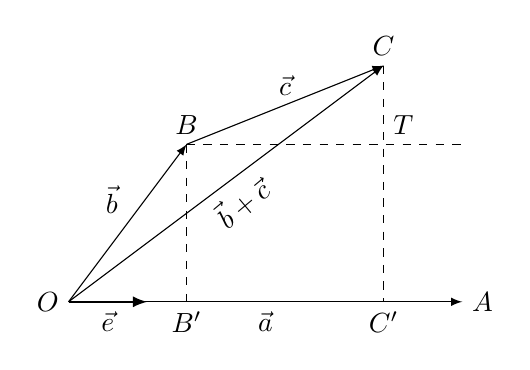
\begin{tikzpicture}
		\coordinate (O) at (0,0) node[anchor=east] at (O) {$O$};
		\coordinate (A) at (5,0) node[anchor=west] at (A) {$A$};
		\coordinate (B) at (1.5,2) node[anchor=south] at (B) {$B$};
		\coordinate (Bp) at (1.5,0) node[anchor=north] at (Bp) {$B'$};
		\coordinate (C) at (4,3) node[anchor=south] at (C) {$C$};
		\coordinate (Cp) at (4,0) node[anchor=north] at (Cp) {$C'$};
		\coordinate (T) at (4,2) node[anchor=west, yshift=0.7em] at (T) {$T$};
		\draw [-latex] (O)--(A) node[midway, below] {$\vec{a}$};
		\draw [-latex, thick] (O)--(1,0) node[midway, below] {$\vec{e}$};
		\draw [-latex] (O)--(B) node[midway, above left] {$\vec{b}$};
		\draw [-latex] (O)--(C) node[midway, below, rotate=40] {$\vec{b}+\vec{c}$};
		\draw [-latex] (B)--(C) node[midway, above] {$\vec{c}$};
		\draw [dashed] (B)--(Bp);
		\draw [dashed] (C)--(Cp);
		\draw [dashed] (B)--(5,2);
	\end{tikzpicture}
	\captionof{figure}{Дистрибутивность скалярного произведения}
\end{minipage}
\begin{align*}
	(\vec{a},\vec{b}+\vec{c})
	 & =(\lvec{OA},\lvec{OC})=|\lvec{OA}|\left(|\lvec{OC}|\cos\angle COA\right)=|\lvec{OA}|\mes_{\vec{e}}\lvec{OC'}
	=|\lvec{OA}|\left(\mes_{\vec{e}}\lvec{OB'}+\mes_{\vec{e}}\lvec{B'C'}\right)=                                    \\
	 & =|\lvec{OA}|\mes_{\vec{e}}\lvec{OB'}+|\lvec{OA}|\mes_{\vec{e}}\lvec{BT}
	=|\lvec{OA}||\lvec{OB}|\cos\angle BOB'+|\lvec{OA}||\lvec{BC}|\cos\angle CBT=(\vec{a},\vec{b})+(\vec{a},\vec{c})\qed
\end{align*}

\props{скалярного произведения}
\begin{enumerate}
	\item{}Коммутативность: $(\forall \vec{a},\vec{b}\in L)\;(\vec{a},\vec{b})=(\vec{b},\vec{a})$
	\item{}Ассоциативность: $(\forall \lambda\in\R,\vec{a},\vec{b}\in L)\;(\lambda\vec{a},\vec{b})=\lambda(\vec{a},\vec{b})$
	\item{}Дистрибутивность: $(\forall \vec{a},\vec{b},\vec{c}\in L)\;(\vec{a},\vec{b}+\vec{c})=(\vec{a},\vec{b})+(\vec{a},\vec{c})$
	\item{}$(\forall \vec{a}\in L)\;(\vec{a},\vec{a})>0\text{, если }\vec{a}\neq \vec{0}\land(\vec{a},\vec{a})=0\text{, если }\vec{a}=\vec{0}$ (тк $(\vec{a},\vec{a})=|\vec{a}|^{2}$)
\end{enumerate}

\theorem

$(\vec{e}_{i})$ --- базис $L^{n}$

$(\alpha_{i})$ --- разложение $\vec{a}$ по этому базису

$(\beta_{i})$ --- разложение $\vec{b}$ по этому базису
\begin{align*}
	(\vec{a},\vec{b})=\sum_{i=1}^{n}\sum_{j=1}^{n}\alpha_{i}\beta_{j}(\vec{e}_{i},\vec{e}_{j})
\end{align*}

\proof
\begin{align*}
	 & (\vec{a},\vec{b})=\left(\sum_{i=1}^{n}\alpha_{i}\vec{e}_{i},\sum_{j=1}^{n}\beta_{j}\vec{e}_{j}\right)
	=\sum_{i=1}^{n}\alpha_{i}\left(\vec{e}_{i},\sum_{j=1}^{n}\beta_{j}\vec{e}_{j}\right)
	=\sum_{i=1}^{n}\alpha_{i}\sum_{j=1}^{n}\beta_{j}(\vec{e}_{i},\vec{e}_{j})
	=\sum_{i=1}^{n}\sum_{j=1}^{n}\alpha_{i}\beta_{j}(\vec{e}_{i},\vec{e}_{j})\qed                            \\
	 & \text{В ДПСК: } (\vec{a},\vec{b})=\sum_{i=1}^{n}\alpha_{i}\beta_{i}
\end{align*}

\end{document}
